\chapter{New middleware architecture}

\section{Design goals and core concepts}

\section{Architecture overview}

The PerLa Middleware is responsible for managing the lifecycle of all devices
connected to the PerLa framework, and for providing a uniform API to interact
with them. Its design revolves around the Functionality Proxy Component
(\texttt{FPC}), a self-contained proxy object that embeds all the logic
required to communicate with a single remote device.  The most prominent trait
of the \texttt{FPC} is its interface, an API that allows PerLa users to
interact with the sensing network through two hardware-agnostic communication
primitives, named get() and set().  Use of this interface neither requires
knowledge of the sensing network, nor of the device that will ultimately
perform the requested operation.

\begin{figure}[h!]
\center
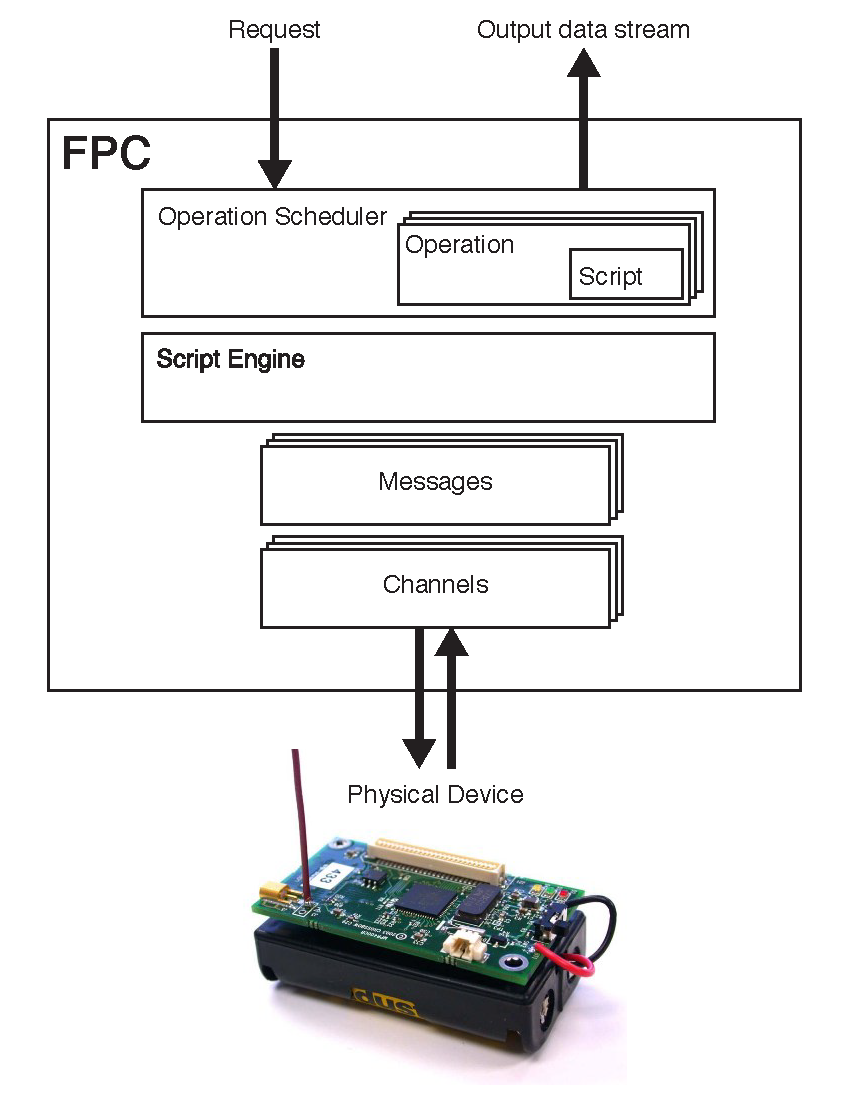
\includegraphics[width=0.6\textwidth]{imgs/fpc.pdf}
\caption{Internal FPC structure}
\label{fig:fpc_overview}
\end{figure}

Each \texttt{FPC} is formed from the composition of various independent
software units, each of which is responsible for the management of a single
aspect of the interaction with the remote device (see
figure~\ref{fig:fpc_overview}). This modular design was chosen to promote
reusability and foster future expandability through composition of
independent objects. The following list contains a synopsis of the modules
that form an \texttt{FPC}:

\begin{itemize}

    \item \textbf{Channel:} A software component capable of performing I/O
    operations. \texttt{Channels} are responsible for managing the
    communication between the PerLa framework and the remote devices;

    \item \textbf{Mapper:} A data marshaller/unmarshaller. \texttt{Mappers}
    allow the \texttt{FPC} to interpret byte streams received from a Channel,
    and to serialize high-level data structures prior to transmission;

    \item \textbf{Script Engine:} An interpreter for executing PerLa
    \texttt{Scripts}, small programs written in a proprietary PerLa scripting
    language, which are used to dynamically bind high level data requests to
    native processing tasks performed on the remote device;

    \item \textbf{Operation Scheduler:} Schedules the execution of concurrent
    data collection operations on the remote device. The scheduler may simulate
    certain operations if the device connected to the FPC is not able to
    perform them natively (e.g., periodic sampling may be simulated by polling
    the remote device at regular intervals).

\end{itemize}

\begin{figure}[h!]
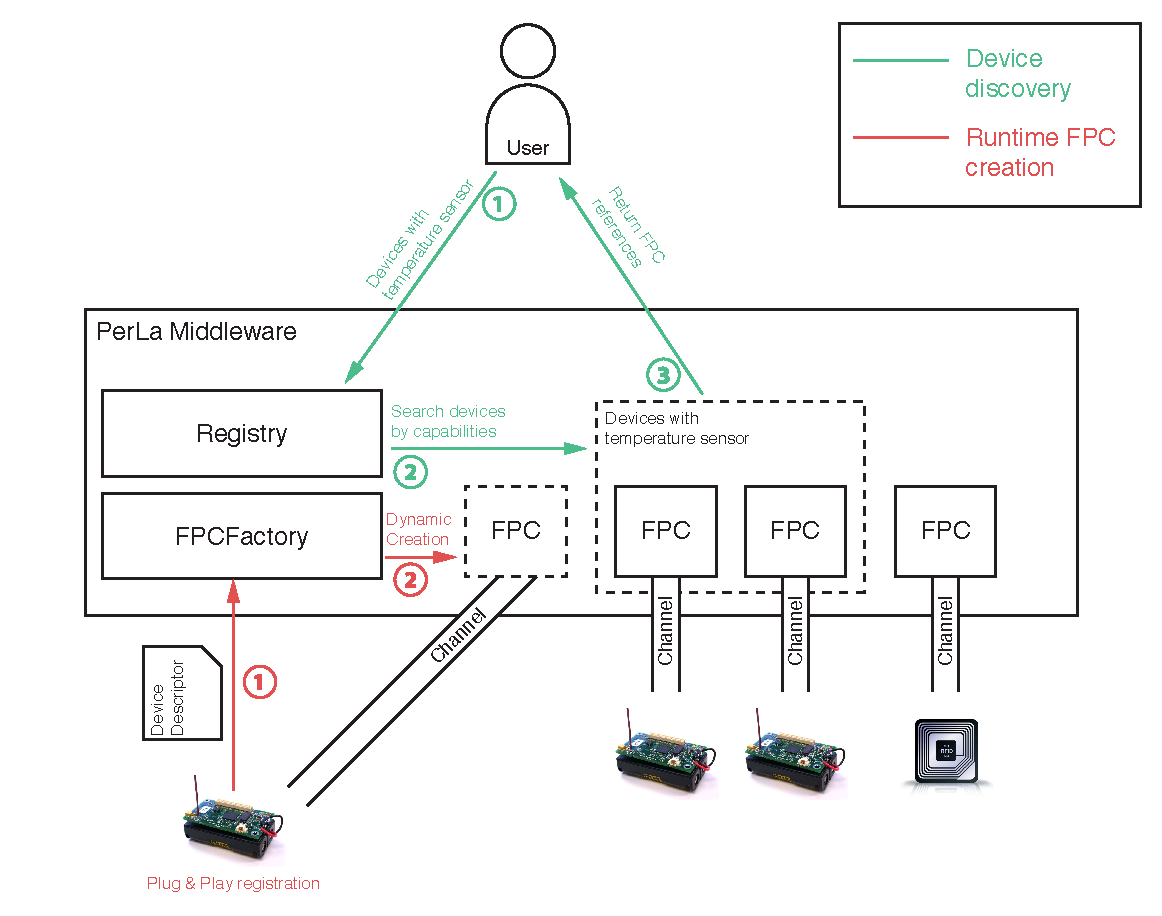
\includegraphics[width=\textwidth]{imgs/middleware_overview.pdf}
\caption{Internal FPC structure}
\label{fig:fpc_overview}
\end{figure}

New \texttt{FPC} objects are instantiated at runtime by the
\texttt{FPCFactory}. The starting point for the creation of an \texttt{FPC} is
the Device Descriptor, an XML document which contains a machine parseable
description of a single sensing device. Device Descriptors are organised in
different sections, each of which defines the configuration of one of the
aforementioned \texttt{FPC} modules. The \texttt{FPCFactory} can receive new
Device Descriptors directly from the node being connected (Plug\&Play
behaviour), or from another entity that acts on behalf of it (off-band
behaviour). The latter approach allows devices which are not capable of
autonomously transmit their Device Descriptor to be registered on the PerLa
Middleware.

A reference to each \texttt{FPC} is stored in the \texttt{Registry}, a
Middleware component that is responsible for maintaining a complete index of
all devices accessible through the PerLa framework. Thanks to the
\texttt{Registry}, PerLa user can discover sensing nodes through
capability-based queries, and retrieve the \texttt{FPC} objects that can be
used to interact with them.

\subsection{Asynchronous interaction paradigm}
\label{sec:newmiddleware.async}

One of the major differences between the New and Classic Middleware
architectures lies in the technique employed to interconnect internal modules
of the PerLa software infrastructure. The New Middleware introduces a fully
asynchronous interaction paradigm based on non-blocking method invocations and
event-driven programming techniques, which deviates profoundly from the
mechanism previously promoted in the Classic design.

\begin{figure}[h!]
    \center
    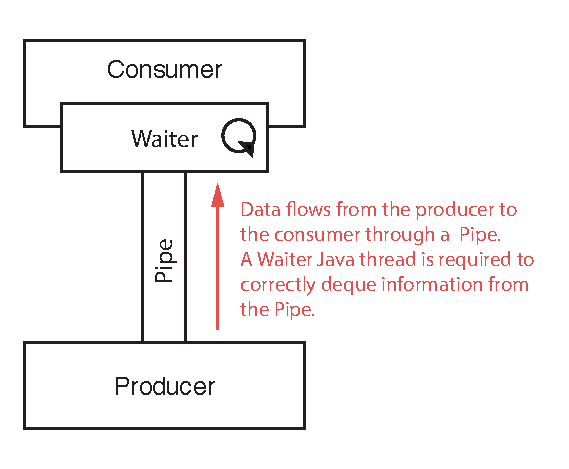
\includegraphics[width=0.5\textwidth]{imgs/pipe_waiter.pdf}
    \caption{A typical \texttt{Pipe}-\texttt{Waiter} connection in the Classic
        PerLa Middleware}
\end{figure}

Within the previous Middleware architecture, a connection between two different
modules was achieved by means of a decoupling element dubbed \texttt{Pipe}, a
one-way message queue designed to shuttle data elements from a software
component to its intended receiver. This system proved to be crucial in the
first development stages of PerLa, as its generic interface allowed the early
designers to experiment with several competing architectures and component
combinations. However, its flexibility came at a cost, both in terms of
performances and API readability. First of all, each \texttt{Pipe} allocated an
initial memory cache of 10 elements. Moreover, the receiving end of a
\texttt{Pipe}, namely the \texttt{Waiter}, was required to instantiate a Java
thread dedicated solely to the reception of data messages. The widespread use
of the \texttt{Pipe}-\texttt{Waiter} paradigm thus led to the proliferation of
threads and to an overuse of memory, which negatively impacted the overall
system efficiency. In addition, the loosely coupled interaction paradigm
promoted by the Classic Middleware resulted in a weak API that lacked intent
and semantic clarity.

The asynchronous, event-driven architecture implemented in the New Middleware
overcomes all aforementioned drawbacks, improving on the overall system
throughput and scalability. Differently from the deprecated
\texttt{Pipe}-driven system, this new design fosters a direct exchange of
information between data producers and data consumers; information is no more
delivered using a mandatory middleman (i.e., the \texttt{Pipe}), but is
explicitly handed over to the intended recipients. This interaction paradigm is
based on the \textit{Hollywood Principle}, a software design methodology whose
principles are summarized by the motto ``\textit{don't call us, we call you}'',
that encourages the development of highly-cohesive, low-coupling APIs, 

\begin{figure}[h!]
\center
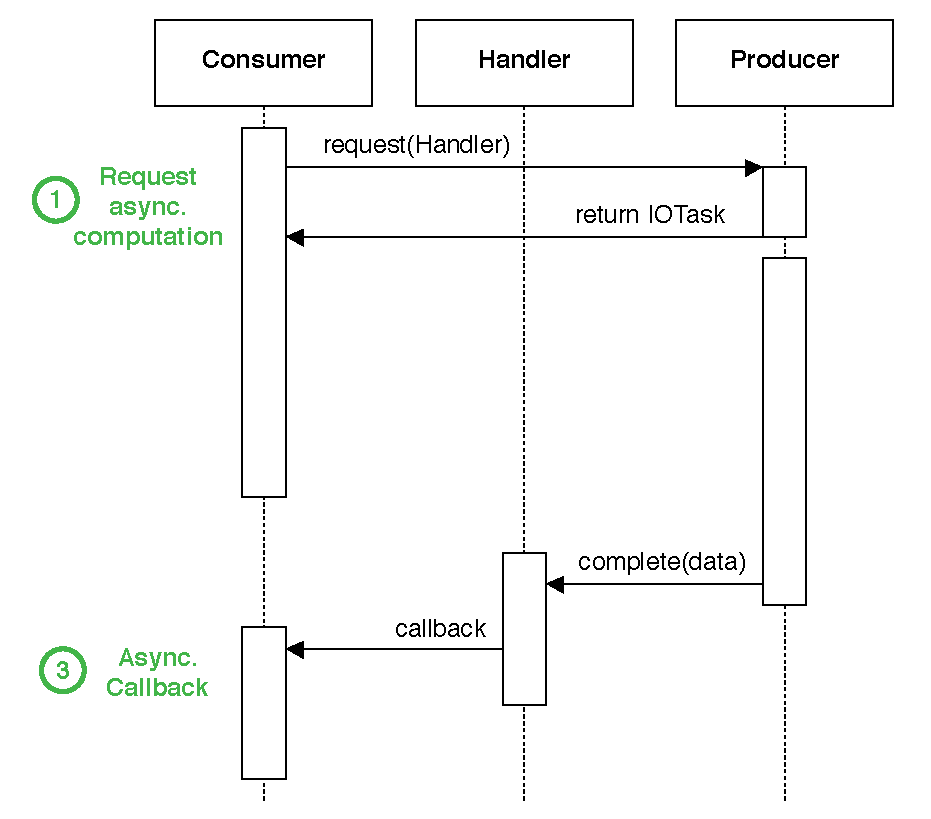
\includegraphics[width=0.8\textwidth]{imgs/async_paradigm.pdf}
\caption{Sequence diagram of an asynchronous method call. Note that the
consumer and the producer continue their execution in parallel.}
\label{fig:async_paradigm}
\end{figure}

Every asynchronous method call in the New PerLa Middleware is identified by the
following characteristics:

\begin{itemize}

    \item \textbf{Does not block:} Calls to an asynchronous method never block;
        control of the execution flow is immediately returned to the caller,
        and the requested computation is executed asynchronously. This
        characteristics reduces the number of Java threads that the caller
        module needs to instantiate;

    \item \textbf{Returns a Task object:} Asynchronous method calls do not
        return the immediate result of a computation. Instead, they return a
        \texttt{Task}, i.e., an object that can be employed to stop the ongoing
        operation or to query its current state of progress;

    \item \textbf{Deferred delivery of results:} The effective Result is
        notified through a \texttt{Handler} function, which is invoked as soon
        as the computation terminates. \texttt{Handler} functions are specified
        upon use of an asynchronous method by the caller module itself.

\end{itemize}

For an in-depth description of the actual asynchronous APIs implemented within
the PerLa Middleware, please refer to chapter~\ref{cha:components}.


\subsection{FPCFactory Plugin System}
\label{sec:newmiddleware.factory}

The new \texttt{FPCFactory} is a modular software entity composed of various
factory components dedicated to the creation of a specific \texttt{FPC} module.
Its design is a significant departure from the original monolithic factory
structure, and allows final users to easily expand the base capabilities of the
PerLa Middleware without modifying its original source code. This modular
architecture, formally called \texttt{FPCFactory} Plugin System, is a direct
implementation of the \textit{Open/Closed} principle: the \texttt{FPCFactory}
is open for extension, as its functionalities can be expanded by adding new
plugins, but closed for modification, since the addition of a new sub-factory
does not require any change to the Middleware's source code.

At the current state of implementation the PerLa Middleware supports three
different \texttt{FPCFactory} plugin types, viz. \texttt{ChannelFactories},
\texttt{IORequestFactories} and \texttt{MapperFactories}, which are responsible
for the creation of new \texttt{Channels}, \texttt{IORequests} and
\texttt{Mappers} respectively (further information on all aforementioned
classes are available in chapter~\ref{cha:components}). Different
implementations of a single plugin type are tasked with creating the same class
of \texttt{FPC} modules; for example, the \texttt{HTTPChannelFactory} and the
\texttt{TinyOSChannelFactory} both create \texttt{Channel} objects, but the
first is used to connect with RESTful web APIs, while the second one interfaces
the PerLa Middleware with a TinyOS network.

The introduction of a new modular \texttt{FPCFactory} Plugin System resulted in
a complete redesign of the Device Descriptor itself, which changed its layout
to accomodate a modular structure that closely follows the new
\texttt{FPCFactory} architecture. The new Device Descriptor is composed of the
following elements:

\begin{itemize}

    \item \textbf{Preamble:} A \lstinline!<device>! XML tag that contains a
        textual description of the endpoint, and a list of XML namespaces used
        to select the various Device Descriptor and \texttt{FPCFactory} plugins
        required for the creation of the \texttt{FPC} object;

    \item \textbf{Attribute declarations:} A list of all the device
        \texttt{Attributes} exposed by the device. It must be enclosed in a
        \lstinline!<attribute>! XML tag;

    \item \textbf{Channel declarations:} This section contains the
        configuration options of all \texttt{Channel} objects required to
        communicate with the remote device. Its contents are parsed and
        interpreted by the \texttt{ChannelFactory} plugins;

    \item \textbf{Message declarations:} A section reserved for the declaration
        of all data structures required to support the interaction with a node
        of the network. Its contents are directly interpreted by the
        \texttt{MapperFactory} plugins for the creation of new \texttt{Message}
        mappers;

    \item \textbf{Request declarations:} This part of the Device Descriptor
        is reserved for the declaration of all \texttt{IORequest} objects
        needed to communicate with a remote device. The helements hereby
        contained are processed by the \texttt{IORequestFactory} plugins;

    \item \textbf{Operation declarations:} This last section of the Device
        Descriptor contains the PerLa \texttt{Scripts} that are used for
        controlling the remote device.

\end{itemize}

\lstset{language=XML}
\begin{lstlisting}[caption={The skeleton of the new XML Device Descriptor.}]
\end{lstlisting}

Moreover, every \texttt{FPCFactory} plugin is responsible for defining the
specific XML syntax to be used in its Device Descriptor section. This feature
endows plugin authors with the possibility to specify the custom set of options
to be used for the creation of their \texttt{FPC} modules. The possibility of
using a custom syntax is key to the new \texttt{FPCFactory} Plugin System,
since different types of plugins may require totally different configuration
options in order to be used or even initialized (e.g., communicating over a
HTTP \texttt{Channel} is considerably different than sending data on a
low-power mesh network).



The New Middleware expands upon the concept of Factory by introducing a modular
Plugin System that improves the flexibility and expandability of PerLa. The
term Factory refers to a widespread design pattern that allows the creation of
new objects without specifying, at compile time, which exact class will be
instantiated. This object creation abstraction is equivalent to a polymorphic
constructor that uses runtime information to create new class instances.
